\section{Properties of blockchain}

All parties in the block chain network have the same copy of the block chain. It's in the best interest of the participant to verify it in order to receive rewards for the network. In a system where each participant owns a copy of a database, we need to prevent addition of illegitimate block. The traditional model requires a central authority which is trusted to be honest to confirm a transaction. If this point of the network is going to be compromised an attacker could cause extensive damage to the system. Blockchain solution eliminates the central authority by distributing the copies of records to the peers, they broadcast changes by forming new blocks and requesting validation based on the rules of the consensus model.  Once validated, the block is added to everyone’s chain. The process is potentially safer than the traditional model, and the middleman agent isn't required, invoking a disruption to the status quo.

\begin{figure}[H]
    \begin{center}
        \begin{minipage}{\linewidth}
            \begin{center}
                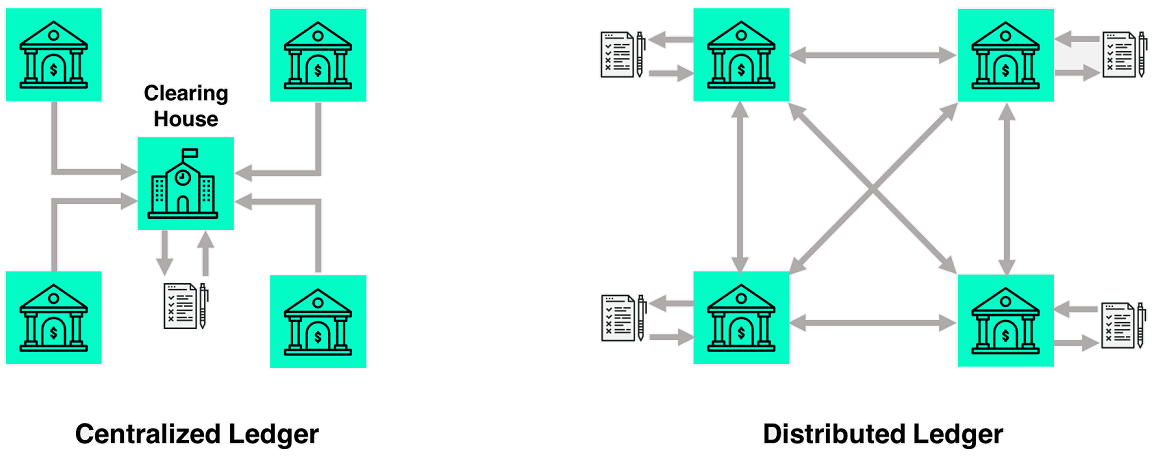
\includegraphics[width=\textwidth,keepaspectratio]{img/centralized_vs_distributed.png}
                \caption{Centralized and distributed ledger \cite{tradeix}}
                \label{obr 1.2.1}
            \end{center}
        \end{minipage}
    \end{center}
\end{figure}

Blockchain is an ongoing chain of blocks records, forming a sequential linked list with hash pointers and separately containing data. A blockchain is typically redundantly distributed across a P2P network, that verifies the integrity of existing blocks and adds new blocks to serve as a distributed database. Verification obeys a set of protocol rules, the codebase. The goal of a blockchain is to be secure by design with a tamper-proof validation of data at a time. We can summary blockchain properties into \cite{Conceptualizing}

\begin{description}
\item[Immutability] (permanent and tamper-proof)  a blockchain is a permanent record of  transactions. Once a block is added, it cannot be altered.  This creates trust in the transaction record.
\item[Security] (trust verification) each block on the blockchain is verified independently via a Consensus model which provide rules for validating a block, and often use a scarce resource (such as computing power) to show proof that adequate effort was made.  In Bitcoin, this is referred to as the mining process.  works without the use of a central authority or an explicit trust-granting agent.
\item[Decentralization] (networked copies) a blockchain is stored in a file that can be accessed and copied by any node on the network.  This creates decentralization.
\end{description}

\section{Asymmetric cryptography}

Asymmetric cryptography, also known as public-key cryptography, is one of the key components of blockchain technology. This form of cryptography allows everyone to verify the integrity of the transaction. Public Key Cryptography is a cryptographic system that relies on a pair of keys, a private key which is kept secret and a public key which is broadcasted out to the network. We can think of a public key as a user name which can be displayed on the internet without any concerns about security. On the other hand, a private key is password that tightly coupled with the user name. It's practically impossible to derive the private key from a public key. 



\begin{figure}[H]
    \begin{center}
        \begin{minipage}{\linewidth}
            \begin{center}
                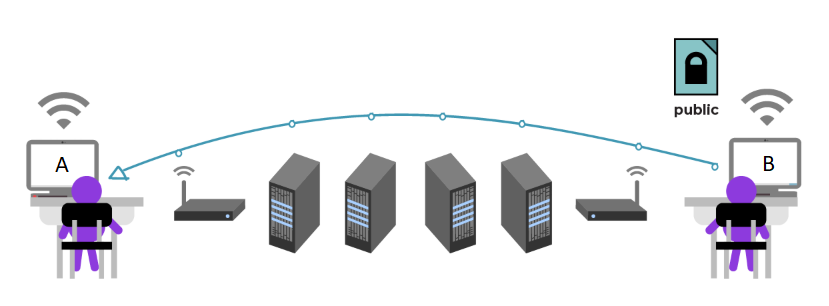
\includegraphics[width=\textwidth,keepaspectratio]{img/asymetric1.png}
                \caption{Sending encrypted message \cite{SSD.EFF.ORG}}
                \label{obr 1.2.1}
            \end{center}
        \end{minipage}
    \end{center}
\end{figure}

If person $A$ wants to send an encrypted message to $B$ to be sure that only $B$ will be able to read it without any intermediates $A$ has to use $B$'s public key to encrypt a message. This message can be send through many computers and not a single one would be able to read the content of the message. Intermediaries such as the email service providers, Internet service providers, and those on their networks—are able to see meta-data this whole time: who is sending what to whom, when, what time it’s received, what the subject line is, that the message is encrypted  \cite{SSD.EFF.ORG}.
Once the message is received by $B$, he has to use his securely stored private key to decrypt the message. 

\begin{figure}[H]
    \begin{center}
        \begin{minipage}{\linewidth}
            \begin{center}
                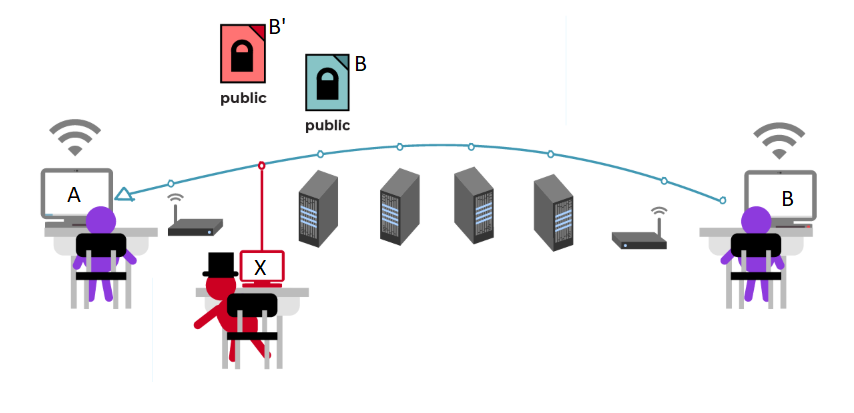
\includegraphics[width=\textwidth,keepaspectratio]{img/asymetric2.png}
                \caption{Sending encrypted message with the man in the middle \cite{SSD.EFF.ORG}}
                \label{obr 1.2.1}
            \end{center}
        \end{minipage}
    \end{center}
\end{figure}

If an intermediary with a bad intention finds a way to convince $A$ to use wrong public key $B'$ to send $B$ a message he can alter or read the message. This attack is called \emph{man in the middle attack} which consists of $X$ creating a keypair $B'$. Once the message has been captured by $X$ he can decrypt the message using his private key for $B'$, read or alter the message and encrypt it using the real $B$ public key and forward it to the recipient. 
This can be avoided by using \emph{fingerprints} or hashes of the public key. Parties that want to have a secured conversation should share their fingerprints of public keys preferably in person or through a different secured channel and verify the public key before encrypting the message.

Using private-public key encryption we can digitally sign a document to verify that the sender is legitimate. The sender $A$ with public key $KV_A$ and private key $KT_A$ signs his message $M$ such that he attaches the result of deciphering of message $M$ with his private key $KT_A$ 

\begin{center}
    $Sig(M) =D_{KTA}(M)$
\end{center}.

The receiver $B$ tests the authenticity of the signature so that he encipherers the signature with public key $KVA$ of the sender – calculates
\begin{center}
    $M'=E_{KVA(Sig(M)}$
\end{center}

and check whether $M = M'$. If $M' \neq M$, then the message was forged or the signature is not genuine. If $M' = M$, then the signature is genuine and the message is unchanged. The only person – the sender $A$ – could create $Sig(M) = D_{KTA}(M)$ for message $M$ since he is the only participant who has private key $KTA$. \cite{OneWayHashFunctions}

Major cryptocurrencies like Bitcoin and Ethereum function using three fundamental pieces of information: the address, associated with a balance and used for sending and receiving funds, and the address’ corresponding public and private keys. The generation of address begins with the generation of a private key. From there, its corresponding public key can be derived using a known algorithm. The address, which can then be used in transactions, is a shorter, representative form of the public key.

The private key is what grants a cryptocurrency user ownership of the funds on a given address. The Blockchain wallet automatically generates and stores private keys for you. When you send from a Blockchain wallet, the software signs the transaction with your private key without actually disclosing it, which indicates to the entire network that you have the authority to transfer the funds on the address you’re sending from.

The security of this system comes from the one-way street that is getting from the private key to the public address. It is not possible to derive the public key from the address; likewise, it is impossible to derive the private key from the public key. 